% This is "sig-alternate.tex" V2.1 April 2013
% This file should be compiled with V2.5 of "sig-alternate.cls" May 2012
%
% This example file demonstrates the use of the 'sig-alternate.cls'
% V2.5 LaTeX2e document class file. It is for those submitting
% articles to ACM Conference Proceedings WHO DO NOT WISH TO
% STRICTLY ADHERE TO THE SIGS (PUBS-BOARD-ENDORSED) STYLE.
% The 'sig-alternate.cls' file will produce a similar-looking,
% albeit, 'tighter' paper resulting in, invariably, fewer pages.
%
% ----------------------------------------------------------------------------------------------------------------
% This .tex file (and associated .cls V2.5) produces:
%       1) The Permission Statement
%       2) The Conference (location) Info information
%       3) The Copyright Line with ACM data
%       4) NO page numbers
%
% as against the acm_proc_article-sp.cls file which
% DOES NOT produce 1) thru' 3) above.
%
% Using 'sig-alternate.cls' you have control, however, from within
% the source .tex file, over both the CopyrightYear
% (defaulted to 200X) and the ACM Copyright Data
% (defaulted to X-XXXXX-XX-X/XX/XX).
% e.g.
% \CopyrightYear{2007} will cause 2007 to appear in the copyright line.
% \crdata{0-12345-67-8/90/12} will cause 0-12345-67-8/90/12 to appear in the copyright line.
%
% ---------------------------------------------------------------------------------------------------------------
% This .tex source is an example which *does* use
% the .bib file (from which the .bbl file % is produced).
% REMEMBER HOWEVER: After having produced the .bbl file,
% and prior to final submission, you *NEED* to 'insert'
% your .bbl file into your source .tex file so as to provide
% ONE 'self-contained' source file.
%
% ================= IF YOU HAVE QUESTIONS =======================
% Questions regarding the SIGS styles, SIGS policies and
% procedures, Conferences etc. should be sent to
% Adrienne Griscti (griscti@acm.org)
%
% Technical questions _only_ to
% Gerald Murray (murray@hq.acm.org)
% ===============================================================
%
% For tracking purposes - this is V2.0 - May 2012

\documentclass{sig-alternate-05-2015}

\begin{document}

\setcopyright{acmcopyright}


% DOI
\doi{10.475/123_4}

% ISBN
\isbn{123-4567-24-567/08/06}


\title{Analysis to Electricity Consumption and Economic Indicators Based on Trajectory Similarity}

\author{ \vspace{-1em}
}

\maketitle

%!TEX root=../sig-alternate-sample.tex


\begin{abstract}
As is widely known, the electronic are closely connected to the economic development. Lots of work has been placed on the regression relationship between the economic metrics and electricity-related indexes, which not focus on the tendency wholly. Obviously, the economic and electricity data can be treated as trajectories composed of points with 
s\end{abstract}

\keywords{ACM proceedings; \LaTeX; text tagging}

%!TEX root=../sig-alternate-sample.tex

\section{Introduction}
China has gone through a rapid economic growth in the past three decades, and economy boosting in east china area has always been a highlight. Ever since, electricity has been a powerful catalyst for social development and economic growth. Empirically, economic fluctuation would cause changes in electricity consumption and electricity consumption can also reflect the economic change. Nowadays, the GDP growth has slowered to blew 7\%, which officially is called "new normal". Economic policies would adjust to this new situation, thus asking energy strategies to change. New situation has raised many command for the research to the relationship between the economic indicators and the electricity consumption. 

Historically, there has been lots of work in the causal relationship between economic growth and electricity consumption, most of which used the regression or statistical method traditionally. Many previous work mainly focused on the simple GDP. The study of the relationship between energy consumption and economic growth started with the seminal work of \cite{kraft:relationship}, in which causality between the energy consumption and GNP growth was found using Granger test. Subsequently, actual circumstances in the developed countries was studied like the United Kingdom, Germany, Italy\cite{yu:causal, erol1987causal}. Due to the boosting prosperity, Asian economy also attracted the eyes of researchers like South Korea and Singapore. The cointegration and error-correction models were also applied to research from the viewpoint of the time-series\cite{glasure1998cointegration}.

But these works cannot focus the similarity of tendency treat the economic development process as a whole. Meanwhile, not only the GDP or GNP but also many other economic indicators in many fields such as industry, investment, etc, have strong ties with the electric power metrics. Also, traditional work researched the whole country, but we all know that regional developmental difference could be so astonishingly large that the result could not reflect the true closeness between electricity and economy.  

From another viewpoint, the economic indicators and electricity consumption can be viewed as time series data, which are similar to the trajectory. A traditional trajectory is a sequence of sample points consisting of geo-location and timestamp. Similarly, both the economic indicators and electricity consumption data consists of the value and timestamp. Therefore, we can compare trajectory similarity using many methods focusing on different characteristics. Our work in this paper would focus on the exploit of internal link between economic indicators and electricity consumption using trajectory similarity, which is much novel comparing to the previous work on the relationship between economic indicators and electricity consumption. 

\begin{figure}[!t]
	\centering
	\vspace{-0.5em}
	
\includegraphics[scale=1]{fig/AreaSim-Example}
	\vspace{-1.5em}
	\caption{AreaSim Example}
	\label{fig:area-exa}
	\vspace{-1.5em}
\end{figure}

To address this problem, we propose a trajectory-similarity framework, which allows us to select the top-k closely relevant indicators using the trajectory similarity and verify the lagging time between indicators and electricity consumption. Firstly, we normalize the indicator data and electricity data to make them comparable. We also proposed a similarity method called AreaSim, which need us to calculate the least area enclosed by two trajectories. Since we seek for the similarity of the shape as to the trajectories, we do not need to focus on the original polygon enclosed by trajectories. As shown in Fig~\ref{fig:area-exa}, the original polygon enclosed by trajectory $T$ and $Q$ is such large that the high similarity between these two trajectories cannot be described. Then, we move the trajectory $Q$ vertically getting a set of candidate trajectory set such as $\{Q_1, Q_2, Q_3, \cdots \}$, and from the candidate set, we can find out one trajectory that has the least area with trajectory $T$. Obviously, it is the least area that we should use to calculate the similarity. Meanwhile, it is known that economic activities would last for some time and affect the related metrics which are measured afterward. As elaborated in Fig~\ref{fig:lag-exa}, we want to compare the shape of trajectory $T$ and $Q$. If we move the $Q$ horizontally, we can get the candidate trajectory set such as $\{Q_1, Q_2, \cdots \}$. From the candidate set, we could find a candidate trajectory such as $Q_2$, which has biggest similarity. The time offset between $Q_2$ and $Q$ is the lagging time that exists in two metrics represented by $T$ and $Q$. 

\begin{figure}[!t]
	\centering
	\vspace{-0.5em}
	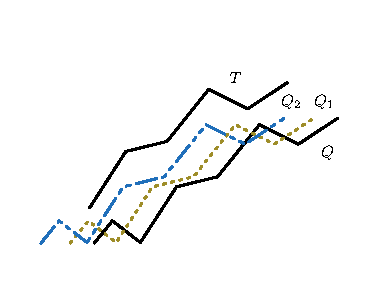
\includegraphics[scale=1]{fig/Lagging-Example}
	\vspace{-1.5em}
	\caption{Lagging Example}
	\label{fig:lag-exa}
	\vspace{-1.5em}
\end{figure}

To summarize, we make the following contributions. 

\vspace{.25em}
\noindent (1) We propose a new similarity function and an efficient framework to compute the trajectory similarity and the lagging time between electricity consumption and economic indicators.

\vspace{.25em}
\noindent (2) We compare different trajectory similarity methods others proposed and implement them correctly. Creatively, we apply these trajectory similarity on the economic data and devise efficient techniques to quicken the computation.  

\vspace{.25em}
\noindent (3) We have conducted an extensive set of experiments on real-world datasets. Instead of focusing on the entire country, we make efforts at the specific provinces. Experimental results show that our algorithm achieves high quality and efficiency. We design various experiments to probe data in east China and get meaningful conclusions.

\vspace{.25em}

The rest of the paper is organized as follows. We formalize our problem in Section~\ref{sec:prem} and introduce our framework in Section~\ref{sec:alg}. Experimental results are provided in Section~\ref{sec:exp}. We review related work in Section~\ref{sec:rel-wor} and conclude the paper in Section~\ref{sec:con}.

%Consequently, the study of the casual relationship between economic indicators and the electricity consumption would shed light on future energy policies, such as the energy conservation, the planning of capacity expansion and the reliable supply of electricity.
%!TEX root=../sig-alternate-sample.tex

% Section Problem Formulation

%\vspace{-1.5em}
\section{Problem Formulation} \label{sec:prem}
In this section, we will formalize our work into a time series similarity question and define the notations that we need in the blow.

Traditionally, the time series of economic indicators and electricity consumption would be analyzed as point series ignoring the shape of lines connecting these points. Before we elaborate the concise similarity problem, we first give a formal definition of a time series. 

\newcommand{\loci}[1]{\ensuremath{p^{#1}}}
\newdef{definition}{Definition}
\begin{definition}
A time series $T$ is a series of data points indexed in time order, i.e., $T=\{\loci{1}, \loci{2}, \cdots, \loci{|T|}\}$, where $\loci{k}$ is a discrete-time data point and |T| is the number of sample points. Discrete-time data point $\loci{k}$ is composed by $\left(D,V\right)$, where $D$ is the date and $V$ is the value.
\end{definition}

Two adjacent data point on $T$ form a line and $T$ has $|T|-1$ lines. As to the electricity consumption and economic indicators data, the time unit is month usually. The broken line connecting the time series data can be analyzed as trajectory since it has a sequence of points. We will refer to the \textbf{broken line} as the \textbf{trajectory}.
%Suppose we have a series of data in \textit{n} months, each monthly data is composed by \textbf{\(date, val\)}, in which $date$ is the month, and $val$ is the value of economic indicator or electricity consumption. A \textit{segment $T$} is a sequence of data points, i.e.$This place is suspicious$, $T=\{\loci{1}, \loci{2}, \cdots, \loci{|T|}\}$,  where $\loci{k}$ is a data point. And $|T|$ is the number of data points in $T$.

Given two trajectories $T$ and $Q$, there is a enclosed polygon if we connect the starting points and . we would use the area of the polygon enclosed by them to evaluate the relevance. It is very obvious to see that the less the enclosed area of these two trajectories is, the more similar the tendency of these two series is. Also, the time interval should be kept the same in two trajectories. The area enclosed by two trajectories can be defined as:

\begin{definition}	
\begin{displaymath}
\textbf{S} = \sum_{k=1}^{n-1}\Delta S_k	
\end{displaymath}
\end{definition}

Each part of the enclosed polygon \textit{$\Delta S_k$} is that the area of shape enclosed by the two segments and vertical coordinates. According to the different tendencies, we can conclude just two cases.
\begin{itemize}
	\item Two segments doesn't intersect. Then, the enclosed part is a trapezoid, of which area is calculated as:
\begin{equation}
	\Delta S_k = \frac{(a + b) * (t_{k+1} - t_k)}{2}
\end{equation}
	\item Two segments intersects. Then, we can treat it as the sum of two triangles.
\begin{equation}
	\Delta S_k = \frac{a * h_i}{2} + \frac{b * h_j}{2}, h_i + h_j = t_{k+1} - t_k 
\end{equation}
\end{itemize} 

Though we have proposed the area of two segments, it cannot be used to evaluate the similarity of two segments. We want to compare the tendency of two indexes. So, case may be that if two lines goes in the same direction but their distance is very long, we still get the much larger area. So, we can move one of the two lines vertically. With different distances, we would get different area, from which the least area is the most appropriate value to reflect the coincide. So, we could use the notation of MINS as the real area.
\begin{equation}
	MINS = \min{\textbf{S}}	
\end{equation}

Given the statistical report, we could know that different indicators exist the time offset. Given two segments, if we move one of them horizontally, we could get different \textbf{MINS}. Among all the results, the time offset corresponding to the least val is a candidate for the real time offset. Once we got the least similarity for economic indicators, we could rank the similarities of these indicators and found the top-k indicators closely connected to the electricity consumption. We can formalize our problem as one top-k problem as follow:
\begin{definition}
	[[[This part, we can put the top-K problem]]]]
\end{definition} 

\begin{equation}
AreaSIM(Q, T) = 1 - \frac{\int_{0}^{n}D_{Q,T}(t)dt}{n}	
\end{equation}

%!TEX root=../sig-alternate-sample.tex

% Section Algorithms
%\vspace{-1em}
\section{Framework} \label{sec:alg}
In this section, we describe a novel top-k algorithm based on the area similarity to find the top-k relevant economic indicators. 
\subsection{Similarity}

While there are several similarity methods, we can compare other empirical methods with our method. 

DTW(Dynamic Time Warping) is an similarity method that do not require two trajectories to be the same length, and it would allow the time shifting by duplicating the previous element.  Time shifting is beneficial for the shape fitting but it is confusing that allow several points to match one point in another trajectory. Empirically, it is unreasonable to owe economic indicators of several months to the sequence of one electricity consumption of one month.
\begin{equation}
	DTW(R, S) = \left\{
	\begin{array}{ll}
		0,  & \text{R and S is empty}  \\
		\infty,  & \text{R or S is empty}  \\
		dist(r1, s1) + min & \{DTW(Rest(R), Rest(S)),  \\
		 DTW(Rest(R), S), & DTW(R, Rest(S))\}, otherwise
	\end{array}
	\right.
\end{equation} 
DTW notates the distance between two trajectories, so we can define the DTWSIM based on the DTW distance:
\begin{definition}
	DTWSIM(R, S) = 1 - $\frac{DTW(R, S)}{min(\text(|R|, |S|)}$
\end{definition}

LCSS(Longest Common SubSequence) model is an efficient model that can deal with the outliers. Not only that LCSS allows different sampling rates, but also it will omit the points, which are too far away from the other points. LCSS is an variant of the edit distance, value of which notates the count of enough close point-pair. We need to input two parameters:
\begin{itemize}
	\item $\sigma$: the offset of two points
	\item $\epsilon$: the matching threshold 
\end{itemize} 
\begin{equation}
	LCSS(R, S)_{\epsilon, \sigma} = \left\{
	\begin{array}{ll}
		0, & \text{R or S is empty} \\
		1 + LCSS_{\epsilon, \sigma}(Head(R), Head(S)), \\
		\text{if $|r_n - s_m| \leq \sigma and |n - m| \leq \epsilon$} \\
		max{LCSS_{\epsilon, \sigma}(Head(R), S), LCSS_{\epsilon, \sigma}(R, Head(S))}, & otherwise
	\end{array}
	\right.
\end{equation}

LCSS notates the count of matching point pair, so we can define the LCSSSIM:
\begin{equation}\label{sim:less}
	LCSSSIM(R,S)=\frac{LCSS_{\epsilon ,\sigma }(R,S)}{\min(R,S)}
\end{equation}

EDR is another variant of edit distance, which define that the cost of a replace, insert, or delete operation is only 1. Instead of omitting the outliers in the LCSS and using the distance directly in DTW, the EDR reduces effect of the outlier by regulating the distance between a pair of elements to two values, 0 and 1. Like DTW, it also conduct the time shifting method for better shape fitting for two trajectories. EDR distance is defined such:
\begin{equation}
	EDR(R, S) = \left\{
	\begin{array}{ll}
		n & \text{if m = 0} \\
		m & \text{if n = 0} \\
		\multicolumn{2}{l}{\text{min\{EDR(Rest(R), Rest(S)) + subcost,}} \\
		\multicolumn{2}{l}{EDR(Rest(R), S) + 1, } \\
		\multicolumn{2}{l}{EDR(R, Rest(S)) + 1\}, otherwise}  
	\end{array}
	\right.
\end{equation}
where subcost = 0 if $|r1 - s1| \leq \epsilon$ and subcost = 1 otherwise.

EDR distance notates the distance between two trajectories, so we can define the similarity of two trajectories $EDRSIM$ as:
\begin{equation}
	EDRSIM=1 - \frac{EDR(R,S)}{min(|R|, |S|)}
\end{equation} 
\subsection{Lagging}
This paper proposes four similarity metrics:DISSIM, DTWSIM, LCSSSIM, EDRSIM. According to the related report, there exist the lagging between the electricity consumption and economic indicators. In order to verify the lagging, we choose part of the time intervals with time offset, and then calculate the most highest similarity value. Meanwhile, we could get the time lag of these metrics. 

%!TEX root=../sig-alternate-sample.tex

\begin{figure*}[!t]
	\vspace{-2em}
	\hspace*{-1em}\subfigure[AreaSim Top One]{
		\hspace*{-1em}\epsfig{figure=fig/area-ele.eps,width=0.18\textwidth\label{fig:AreaSim}}
	}
	\hspace*{-1em}\subfigure[DTW Top One]{
		\hspace*{-1em}\epsfig{figure=fig/dtw_ele.eps,width=0.18\textwidth\label{fig:DtwSim}}
	}
	\hspace*{-1em}\subfigure[LCSS Top One]{
		\hspace*{-1em}\epsfig{figure=fig/lcss-ele.eps,width=0.18\textwidth\label{fig:LcssSim}}
	}
	\hspace*{-1em}\subfigure[EDR Top One]{
		\hspace*{-1em}\epsfig{figure=fig/edr-ele.eps,width=0.18\textwidth\label{fig:EdrSim}}
	}
	\vspace{-1.5em}
	\caption{Indicators Most Close to Electricity Consumption in Different Methods. \label{fig:closeindi}}
	\vspace{-1.5em}
\end{figure*}

\section{Experiments} \label{sec:exp}
\subsection{Data Preprocessing}
Different data source supply data with different dimensions. So, we must normalize the data to make them comparable. 
Given a line $S = [(d_1, v_1), \cdots, (d_n, v_n)]$, we can normalize its value using the Min-Max scaling method:
\begin{equation}
	Norm(S) = [(d_1, \frac{v_1 - v_min}{v_max - v_min}), \cdots, (d_n, \frac{v_n - v_min}{v_max - v_min})]
\end{equation}

Normalization is recommended so that the distance between two lines is invariant to value scaling and shifting. In the next part, we will refer the $S$ as $Norm(S)$. 

We have prepared two categories of dataset: economic indicators and the electricity consumption. The first dataset is crawled from the website of National Bureau of Statistics of China. It consists of various of economic indicators monthly in consumer price, industry, fixed assets investment and domestic trading etc, that lasts about recent fifteen years. The second dataset is about the electricity consumption of each day in the east China, which includes Anhui, Fujian, Shanghai, Jiangsu, Zhejiang. In order to ensure the comparability, we sum the daily record of electricity consumption into one new record representing the electricity consumption of the corresponding month. 

We implemented the proposed similarity method as described in the previous sections and presented the experimental results. Our experiments were taken on a MAC OS X at 2.7 GHz with 8GB RAM.
\subsection{Similarity}
Firstly, we will compare the top 10 indicators that mostly close to the electricity consumption. Table~\ref{tab:topindi} shows the top-ten indicators in Anhui Provinces. We could use the Jaccard similarity to evaluate how the results of different methods are relevant. Given set A and B, 
\begin{equation}
	Jaccard(A, B) = \frac{\texttt{|A intersect B|}}{\texttt{|A union B|}}
\end{equation} 
where the $|A|$ notates the count of element in set $A$. Obviously, the value would increase if there are more elements overlapping in these two sets. We could use the DTW method as baseline to evaluate the Jaccard similarity between the results of these methods in different provinces. From the figure~\ref{fig:Jaccard}, we can see that in the top ten indicators, the jaccard similarity of DTW and other methods lie from 0.25 to 0.43, espically the Zhejiang Province, of which results are higher than other provinces. The fact that we can get same indicators in the top ten indicators gives a strong support to the viewpoint that these indicators have a relationship with the electricity consumption.


%\begin{figure}
%	\centering
%	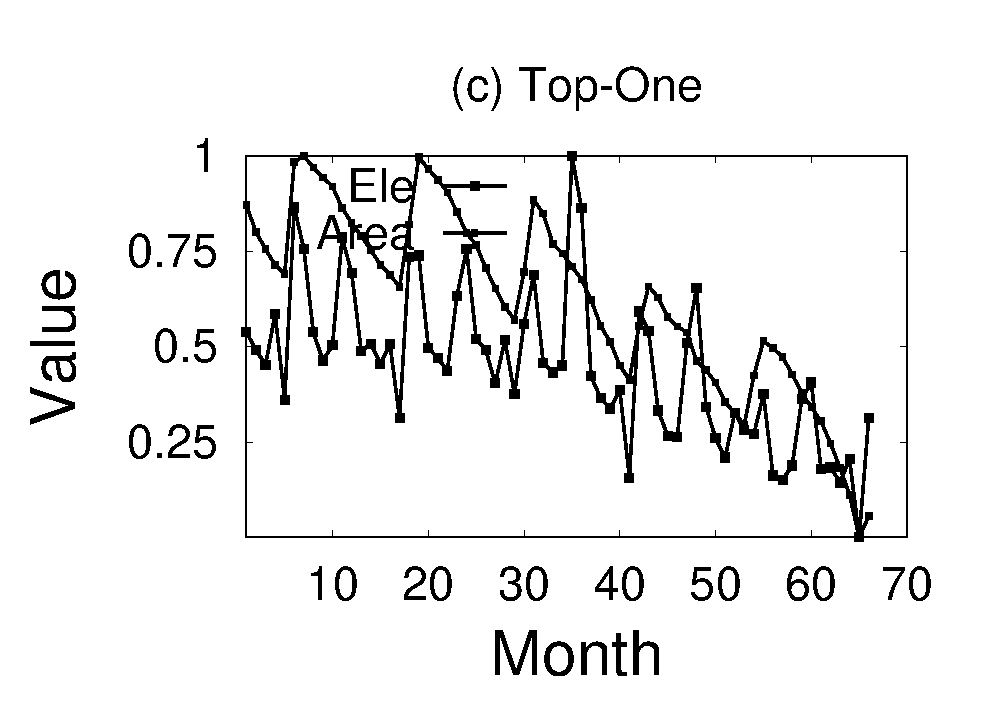
\includegraphics[height=1in, width=0.9in]{area-ele}
%	\caption{AreaSim Top One}
%	\label{fig:AreaSim}
%\end{figure}

%\begin{figure}
%	\centering
%	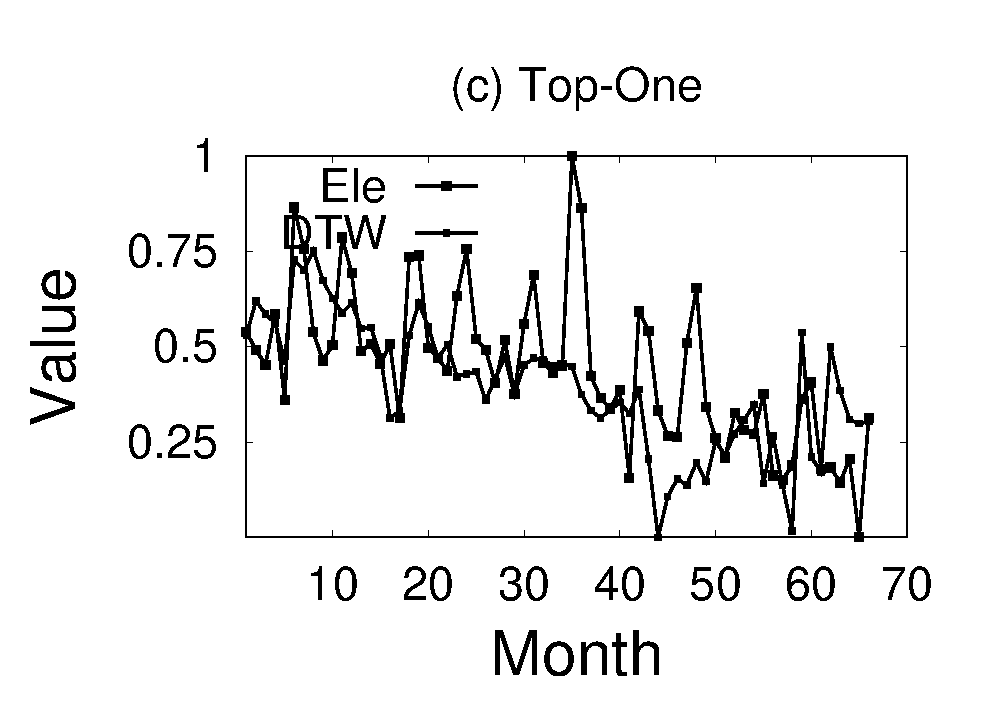
\includegraphics[height=1in, width=0.9in]{dtw_ele}
%	\caption{DTW Top One}
%	\label{fig:DTW}	
%\end{figure}
%
%\begin{figure}
%	\centering
%	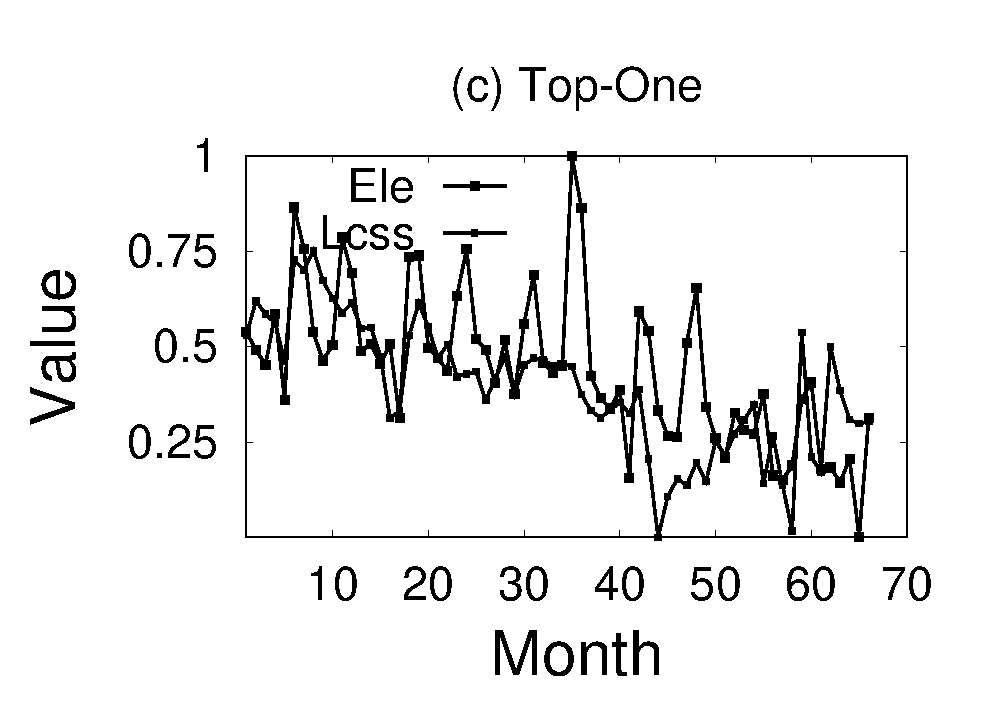
\includegraphics[height=1in, width=0.9in]{lcss-ele}
%	\caption{LCSS Top One}
%	\label{fig:LCSS}
%\end{figure}
%
%\begin{figure}
%	\centering
%	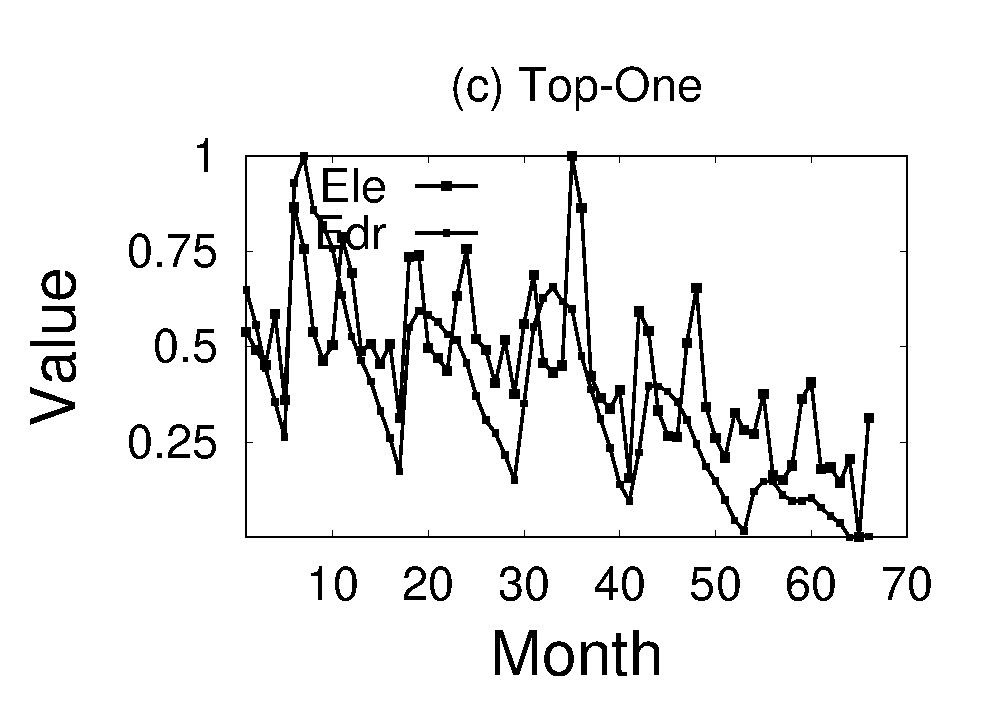
\includegraphics[height=1in, width=0.9in]{edr-ele}
%	\caption{EDR Top One}
%	\label{fig:EDR}
%\end{figure}

\begin{figure}
	\centering
	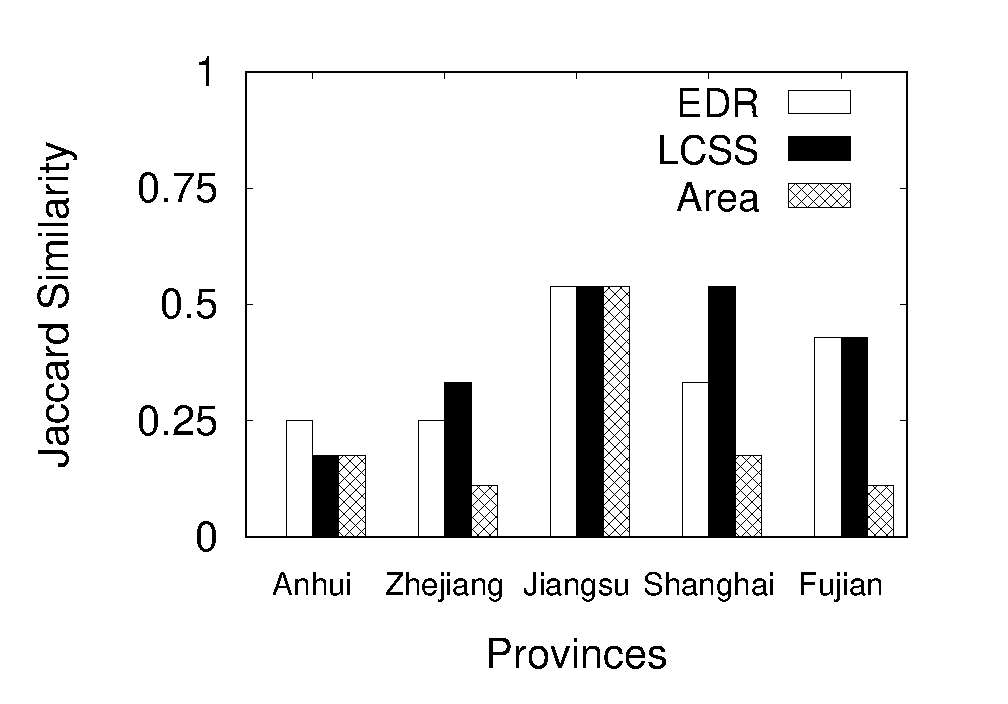
\includegraphics[height=1in, width=0.9in]{fig/dtw_jaccard_similarity}
	\caption{Jaccard Similarity Based on DTW}
	\label{fig:Jaccard}
\end{figure}

\begin{table*}
\centering
\caption{Top 10 Relevant Indicators}
\label{tab:topindi}

\begin{tabular}{|p{3cm}|c|p{3cm}|c|p{3cm}|c|p{3cm}|c|} \hline
	\multicolumn{2}{|c|}{DTWSIM} & \multicolumn{2}{|c|}{LCSSSIM} &\multicolumn{2}{|c|}{EDRSIM} & \multicolumn{2}{|c|}{AreaSIM}\\ \hline
	Construction area of commercial premises\_Cumulative growth(\%) & 0.8944 & The purchase of equipment and instruments in fixed assets investment\_cumulative growth(\%) & 0.9104 & The purchase of equipment and instruments in fixed assets investment\_cumulative growth(\%)& 0.9516 & Residential construction area\_cumulative growth(\%)& 0.8822\\ \hline
	Stock\_cumulative growth(\%) & 0.8930 & Commercial housing construction are\_cumulative growth(\%) & 0.8529 & Commercial housing construction are\_cumulative growth(\%) & 0.9104 & Commercial housing construction are\_cumulative growth(\%) & 0.8817\\ \hline
	Residential construction area\_cumulative growth(\%) & 0.8908 & The amount of investment in fixed assets\_cumulative growth(\%)& 0.8507 & The amount of investment in fixed assets\_cumulative growth(\%) & 0.9032
 & Value added tax payable\_cumulative growth(\%) & 0.8804\\ \hline
	Real estate construction area\_cumulative growth(\%) & 0.8890 &Total current assets\_cumulative growth(\%) & 0.8382 & Total current assets\_cumulative growth(\%) & 0.8955 & The finished product\_cumulative growth(\%) & 0.8787\\ \hline
	Construction area of commercial housing\_Cumulative growth(\%) & 0.8884 & Management Expenses\_Cumulative growth(\%) & 0.8382
& The finished product\_Cumulative Growth(\%) & 0.8955 & Residential construction area\_Cumulative growth(\%) & 0.8749\\ \hline
	Taxes and surcharges of principal operations\_Cumulative growth(\%) & 0.8884 & Accounts Receivable \_ Cumulative Growth (\%) &0.8235 & Accounts Receivable \_ Cumulative Growth (\%) & 0.8805 & Investment in fixed assets completed \_ cumulative growth (\%) & 0.8676
\\ \hline
	Total Assets \_ Cumulative Growth (\%) & 0.8854 & Finished products\_Cumulative growth& 0.8235& Management Expenses\_Cumulative growth&0.8805 & Construction area of office buildings\_Growth(\%) &0.8623\\ \hline
	The purchase of equipment and instruments in fixed assets investment\_cumulative growth(\%) & 0.8841 &Total losses of loss-making enterprises\_Cumulative growth(\%) & 0.8235 &Total losses of loss-making enterprises\_Cumulative growth(\%)&0.8805 &Total losses of loss-making enterprises\_Cumulative growth(\%) &0.8618\\ \hline
	Accounts Receivable \_ Cumulative Growth (\%)& 0.8836& Completed area of commercial premises \_ Cumulative growth (\%) & 0.8235&Residential construction area\_cumulative growth(\%) & 0.8805 &Accounts Receivable \_ Cumulative Growth (\%)& 0.8559\\ \hline
	Total Liabilities \_ Cumulative Growth (\%)& 0.8830 & Residential construction area\_cumulative growth(\%)&0.8088 & Interest Expenditure \_ Cumulative Growth (\%)&0.8805 & The purchase of equipment and instruments in fixed assets investment\_cumulative growth(\%) & 0.8521\\ \hline
\end{tabular}
\end{table*}

\subsection{Lagging}
We have the dataset of electricity consumption and economic indicators lasting for sixty seven months. As is known, economic activities has 
periodicity, which is usually less than one year. Meanwhile, most of our economic indicators are evaluated monthly, so we should view one month as time unit. Taking our data as time series, We extract the middle part of our data intercepting the first last twelve month. And then, keeping the length of electricity consumption data, we move the economic indicator data forward and backward, getting different similarity, from which we could get the largest similarity. The moving month responding to the largest similarity is the lagging time offset we are seeking for. From the fig~\ref{fig:lagdis}, we can see that, different provinces has different lagging distribution.
 
Different lagging time offsets has different instructions for prediction of economic tendency and electricity consumption. The negative lagging time-offset value means that the current electricity consumption has a closer relationship with the economic indicators if we chose the later economic indicators. Therefore, we can predict the later economic indicators using current electricity consumption. Otherwise, if the lagging time-offset value is positive, we can predict the electricity consumption using current economic indicators.   
\begin{figure}
	\centering
	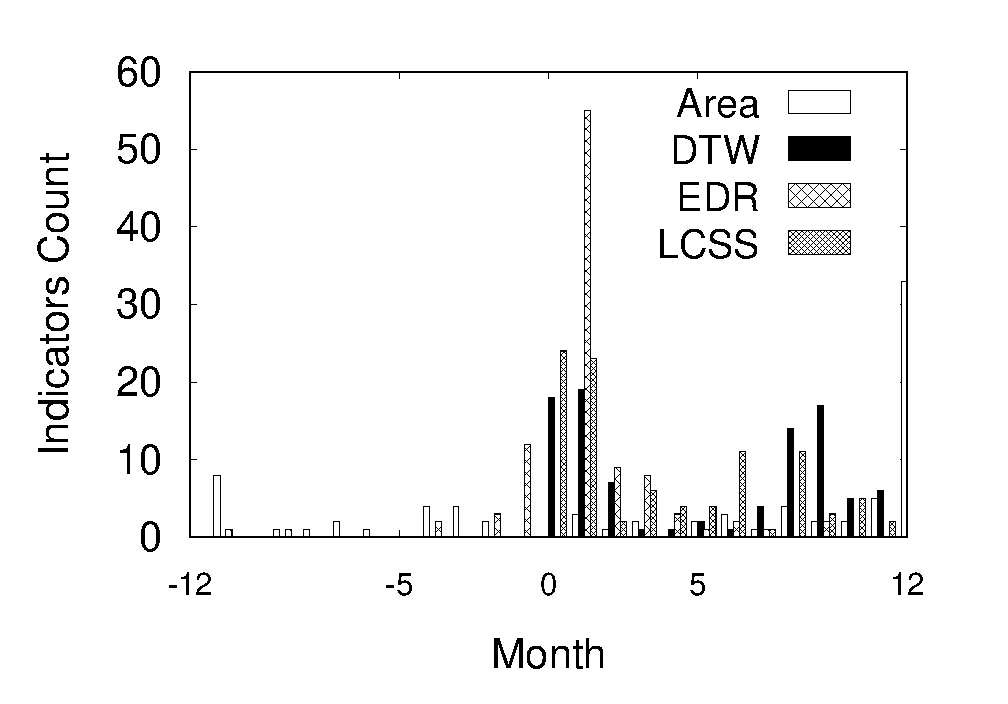
\includegraphics[height=1in, width=2in]{fig/anhui_lag_dis}
	\caption{Anhui Lagging Time Distribution}
	\label{fig:anhui_lag}
\end{figure}

\begin{figure}
	\centering
	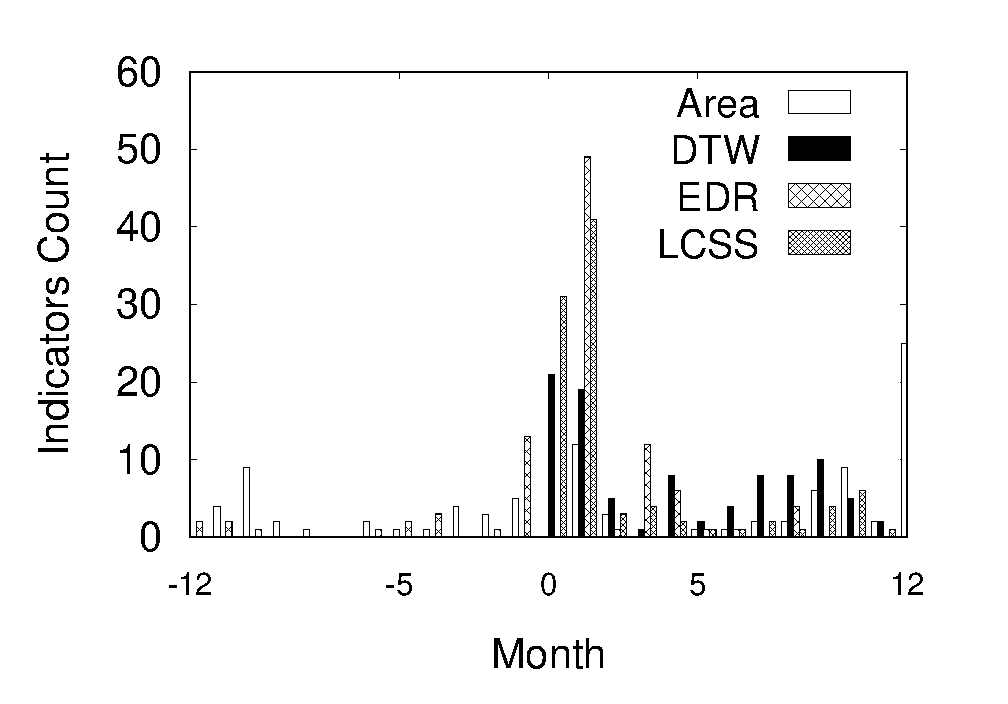
\includegraphics[height=1in, width=2in]{fig/fujian_lag_dis}
	\caption{Fujian Lagging Time Distribution}
	\label{fig:fujian_lag}
\end{figure}

\begin{figure}
	\centering
	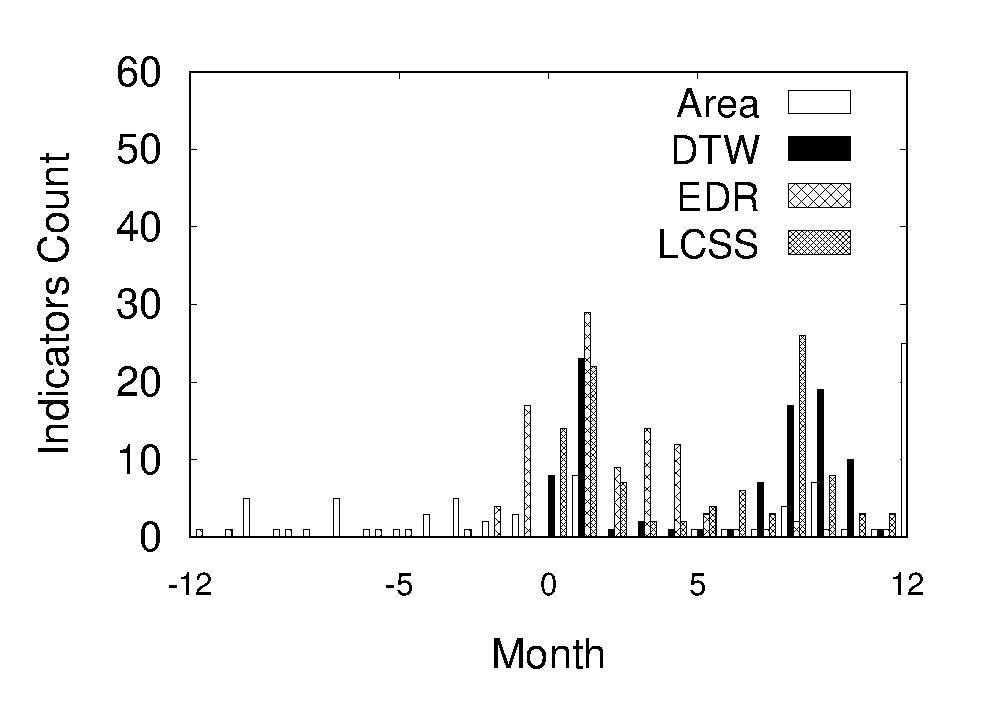
\includegraphics[height=1in, width=2in]{fig/jiangsu_lag_dis}
	\caption{Jiangsu Lagging Time Distribution}
	\label{fig:jiangsu_lag}
\end{figure}

\begin{figure}
	\centering
	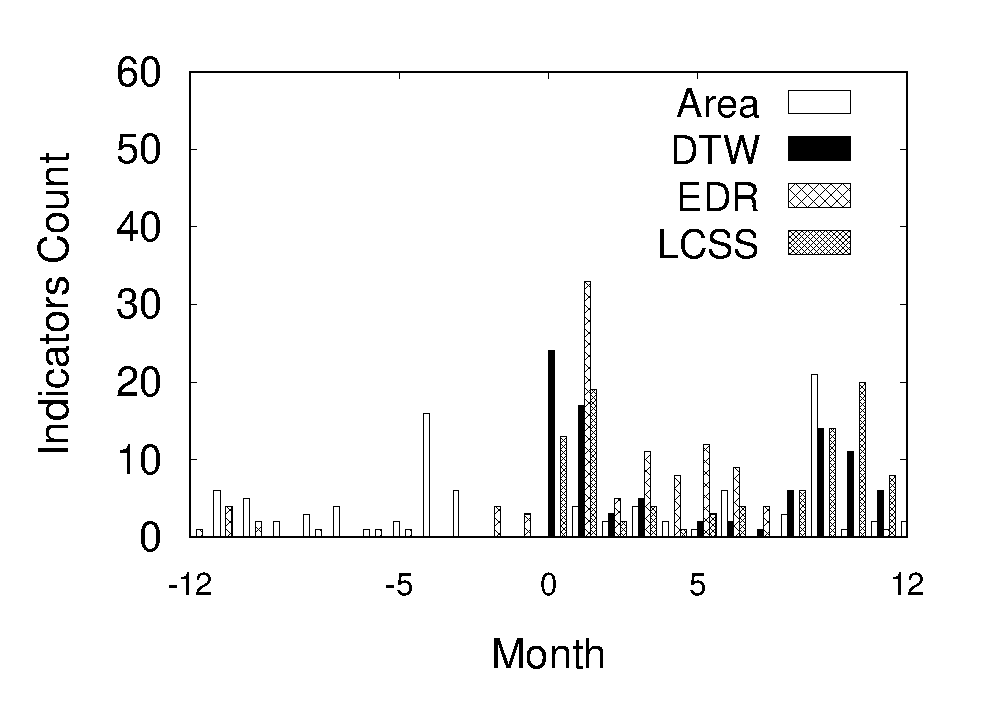
\includegraphics[height=1in, width=2in]{fig/shanghai_lag_dis}
	\caption{Shanghai Lagging Time Distribution}
	\label{fig:shanghai_lag}
\end{figure}

\begin{figure}
	\centering
	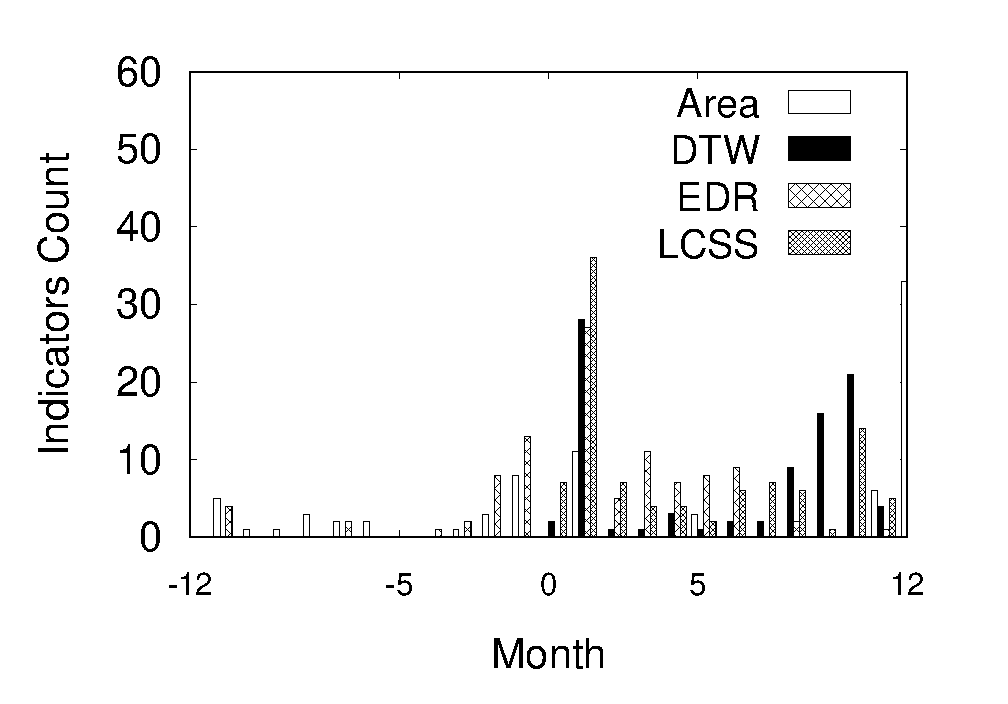
\includegraphics[height=1in, width=2in]{fig/zhejiang_lag_dis}
	\caption{Zhejiang Lagging Time Distribution}
	\label{fig:zhejiang_lag}
\end{figure}
%!TEX root=../sig-alternate-sample.tex

\section{Conclusion}
The time series of economic indicators and electricity consumption would be viewed as a segment. We should evaluate the correlation of economic indicators with electricity consumption through the similarity between the two segments like in Fig 1.[[[[[Here , we should  put one Picture of two examples]]]]] 


\bibliographystyle{abbrv}
\bibliography{sigproc}  % sigproc.bib is the name of the Bibliography in this case
\end{document}
